% Created by tikzDevice version 0.5.3 on 2011-05-02 14:31:11
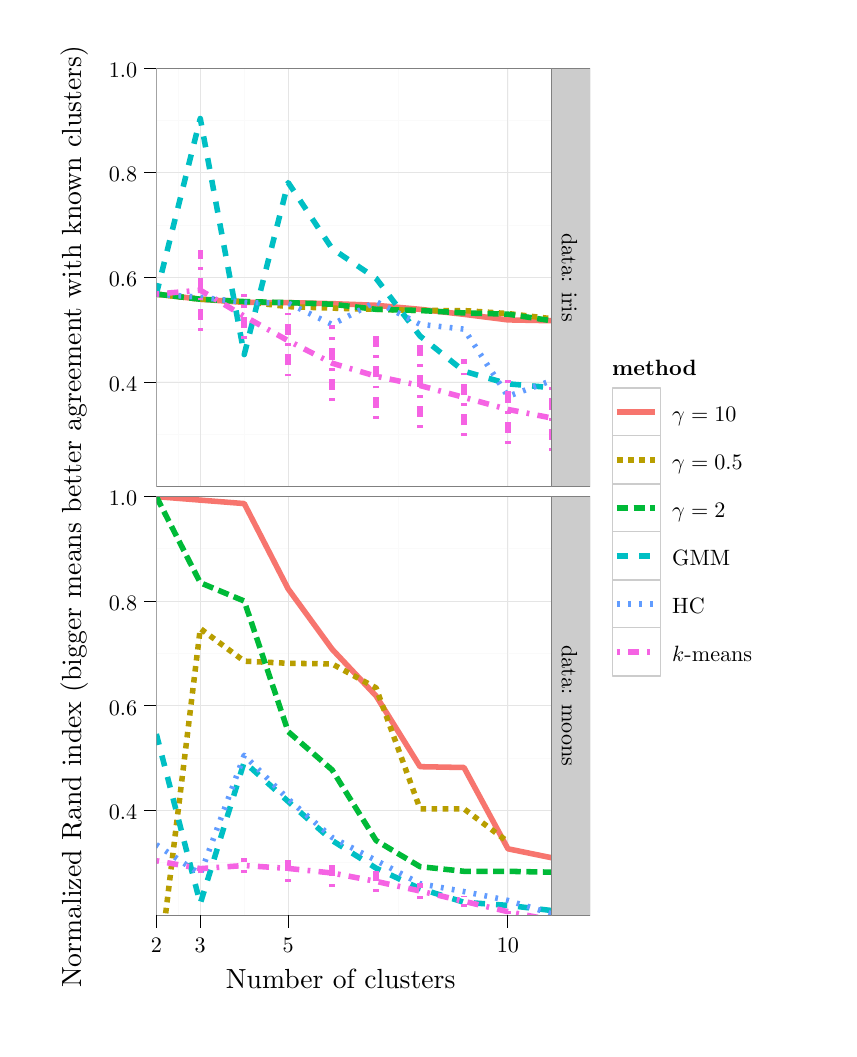
\begin{tikzpicture}[x=1pt,y=1pt]
\draw[color=white,opacity=0] (0,0) rectangle (289.08,361.35);
\begin{scope}
\path[clip] (  0.00,  0.00) rectangle (289.08,361.35);
\end{scope}
\begin{scope}
\path[clip] (  0.00,  0.00) rectangle (289.08,361.35);
\end{scope}
\begin{scope}
\path[clip] (  0.00,  0.00) rectangle (289.08,361.35);
\end{scope}
\begin{scope}
\path[clip] (  0.00,  0.00) rectangle (289.08,361.35);
\end{scope}
\begin{scope}
\path[clip] (  0.00,  0.00) rectangle (289.08,361.35);
\end{scope}
\begin{scope}
\path[clip] (  0.00,  0.00) rectangle (289.08,361.35);
\end{scope}
\begin{scope}
\path[clip] (  0.00,  0.00) rectangle (289.08,361.35);
\end{scope}
\begin{scope}
\path[clip] (  0.00,  0.00) rectangle (289.08,361.35);
\end{scope}
\begin{scope}
\path[clip] (  0.00,  0.00) rectangle (289.08,361.35);
\end{scope}
\begin{scope}
\path[clip] (  0.00,  0.00) rectangle (289.08,361.35);
\end{scope}
\begin{scope}
\path[clip] (  0.00,  0.00) rectangle (289.08,361.35);
\end{scope}
\begin{scope}
\path[clip] (  0.00,  0.00) rectangle (289.08,361.35);
\end{scope}
\begin{scope}
\path[clip] (  0.00,  0.00) rectangle (289.08,361.35);
\end{scope}
\begin{scope}
\path[clip] (  0.00,  0.00) rectangle (289.08,361.35);
\end{scope}
\begin{scope}
\path[clip] (  0.00,  0.00) rectangle (289.08,361.35);
\end{scope}
\begin{scope}
\path[clip] (  0.00,  0.00) rectangle (289.08,361.35);
\end{scope}
\begin{scope}
\path[clip] (  0.00,  0.00) rectangle (289.08,361.35);
\end{scope}
\begin{scope}
\path[clip] (  0.00,  0.00) rectangle (289.08,361.35);
\end{scope}
\begin{scope}
\path[clip] (  0.00,  0.00) rectangle (289.08,361.35);
\end{scope}
\begin{scope}
\path[clip] (  0.00,  0.00) rectangle (289.08,361.35);
\end{scope}
\begin{scope}
\path[clip] (  0.00,  0.00) rectangle (289.08,361.35);

\draw[fill opacity=0.00,draw opacity=0.00,] (  0.00,  0.00) rectangle (289.08,361.35);
\end{scope}
\begin{scope}
\path[clip] (  0.00,  0.00) rectangle (289.08,361.35);
\end{scope}
\begin{scope}
\path[clip] (  0.00,  0.00) rectangle (289.08,361.35);
\end{scope}
\begin{scope}
\path[clip] (  0.00,  0.00) rectangle (289.08,361.35);
\end{scope}
\begin{scope}
\path[clip] (  0.00,  0.00) rectangle (289.08,361.35);
\end{scope}
\begin{scope}
\path[clip] (  0.00,  0.00) rectangle (289.08,361.35);
\end{scope}
\begin{scope}
\path[clip] (  0.00,  0.00) rectangle (289.08,361.35);
\definecolor[named]{drawColor}{rgb}{0.00,0.00,0.00}

\node[color=drawColor,anchor=base,inner sep=0pt, outer sep=0pt, scale=  1.00] at (112.89, 14.45) {Number of clusters%
};
\end{scope}
\begin{scope}
\path[clip] (  0.00,  0.00) rectangle (289.08,361.35);
\end{scope}
\begin{scope}
\path[clip] (  0.00,  0.00) rectangle (289.08,361.35);
\end{scope}
\begin{scope}
\path[clip] (  0.00,  0.00) rectangle (289.08,361.35);
\definecolor[named]{drawColor}{rgb}{0.00,0.00,0.00}

\node[rotate= 90.00,color=drawColor,anchor=base,inner sep=0pt, outer sep=0pt, scale=  1.00] at ( 19.11,184.81) {Normalized Rand index (bigger means better agreement with known clusters)%
};
\end{scope}
\begin{scope}
\path[clip] (  0.00,  0.00) rectangle (289.08,361.35);
\end{scope}
\begin{scope}
\path[clip] (  0.00,  0.00) rectangle (289.08,361.35);
\end{scope}
\begin{scope}
\path[clip] (  0.00,  0.00) rectangle (289.08,361.35);
\end{scope}
\begin{scope}
\path[clip] ( 22.72,346.90) rectangle ( 46.29,346.90);
\end{scope}
\begin{scope}
\path[clip] (  0.00,  0.00) rectangle (289.08,361.35);
\end{scope}
\begin{scope}
\path[clip] ( 22.72,346.90) rectangle ( 46.29,346.90);
\end{scope}
\begin{scope}
\path[clip] (  0.00,  0.00) rectangle (289.08,361.35);
\end{scope}
\begin{scope}
\path[clip] (  0.00,  0.00) rectangle (289.08,361.35);
\end{scope}
\begin{scope}
\path[clip] (  0.00,  0.00) rectangle (289.08,361.35);
\end{scope}
\begin{scope}
\path[clip] ( 22.72,192.09) rectangle ( 46.29,195.70);
\end{scope}
\begin{scope}
\path[clip] (  0.00,  0.00) rectangle (289.08,361.35);
\end{scope}
\begin{scope}
\path[clip] (  0.00,  0.00) rectangle (289.08,361.35);
\end{scope}
\begin{scope}
\path[clip] (  0.00,  0.00) rectangle (289.08,361.35);
\end{scope}
\begin{scope}
\path[clip] ( 22.72, 40.89) rectangle ( 46.29, 40.89);
\end{scope}
\begin{scope}
\path[clip] (  0.00,  0.00) rectangle (289.08,361.35);
\end{scope}
\begin{scope}
\path[clip] ( 22.72, 22.72) rectangle ( 46.29, 40.89);
\end{scope}
\begin{scope}
\path[clip] (  0.00,  0.00) rectangle (289.08,361.35);
\end{scope}
\begin{scope}
\path[clip] ( 22.72, 22.72) rectangle ( 46.29, 22.72);
\end{scope}
\begin{scope}
\path[clip] (  0.00,  0.00) rectangle (289.08,361.35);
\end{scope}
\begin{scope}
\path[clip] ( 46.29,346.90) rectangle ( 46.29,346.90);
\end{scope}
\begin{scope}
\path[clip] (  0.00,  0.00) rectangle (289.08,361.35);
\end{scope}
\begin{scope}
\path[clip] ( 46.29,346.90) rectangle ( 46.29,346.90);
\end{scope}
\begin{scope}
\path[clip] (  0.00,  0.00) rectangle (289.08,361.35);
\end{scope}
\begin{scope}
\path[clip] ( 46.29,195.70) rectangle ( 46.29,346.90);
\end{scope}
\begin{scope}
\path[clip] (  0.00,  0.00) rectangle (289.08,361.35);
\end{scope}
\begin{scope}
\path[clip] ( 46.29,192.09) rectangle ( 46.29,195.70);
\end{scope}
\begin{scope}
\path[clip] (  0.00,  0.00) rectangle (289.08,361.35);
\end{scope}
\begin{scope}
\path[clip] ( 46.29, 40.89) rectangle ( 46.29,192.09);
\end{scope}
\begin{scope}
\path[clip] (  0.00,  0.00) rectangle (289.08,361.35);
\end{scope}
\begin{scope}
\path[clip] ( 46.29, 40.89) rectangle ( 46.29, 40.89);
\end{scope}
\begin{scope}
\path[clip] (  0.00,  0.00) rectangle (289.08,361.35);
\end{scope}
\begin{scope}
\path[clip] ( 46.29, 22.72) rectangle ( 46.29, 40.89);
\end{scope}
\begin{scope}
\path[clip] (  0.00,  0.00) rectangle (289.08,361.35);
\end{scope}
\begin{scope}
\path[clip] ( 46.29, 22.72) rectangle ( 46.29, 22.72);
\end{scope}
\begin{scope}
\path[clip] (  0.00,  0.00) rectangle (289.08,361.35);
\end{scope}
\begin{scope}
\path[clip] ( 46.29,346.90) rectangle (189.23,346.90);
\end{scope}
\begin{scope}
\path[clip] (  0.00,  0.00) rectangle (289.08,361.35);
\end{scope}
\begin{scope}
\path[clip] ( 46.29,346.90) rectangle (189.23,346.90);
\end{scope}
\begin{scope}
\path[clip] (  0.00,  0.00) rectangle (289.08,361.35);
\end{scope}
\begin{scope}
\path[clip] ( 46.29,195.70) rectangle (189.23,346.90);
\end{scope}
\begin{scope}
\path[clip] (  0.00,  0.00) rectangle (289.08,361.35);
\end{scope}
\begin{scope}
\path[clip] ( 46.29,192.09) rectangle (189.23,195.70);
\end{scope}
\begin{scope}
\path[clip] (  0.00,  0.00) rectangle (289.08,361.35);
\end{scope}
\begin{scope}
\path[clip] ( 46.29, 40.89) rectangle (189.23,192.09);
\end{scope}
\begin{scope}
\path[clip] (  0.00,  0.00) rectangle (289.08,361.35);
\end{scope}
\begin{scope}
\path[clip] ( 46.29, 40.89) rectangle (189.23, 40.89);
\end{scope}
\begin{scope}
\path[clip] (  0.00,  0.00) rectangle (289.08,361.35);
\end{scope}
\begin{scope}
\path[clip] (  0.00,  0.00) rectangle (289.08,361.35);
\end{scope}
\begin{scope}
\path[clip] (  0.00,  0.00) rectangle (289.08,361.35);
\end{scope}
\begin{scope}
\path[clip] ( 46.29, 22.72) rectangle (189.23, 22.72);
\end{scope}
\begin{scope}
\path[clip] (  0.00,  0.00) rectangle (289.08,361.35);
\end{scope}
\begin{scope}
\path[clip] (189.23,346.90) rectangle (189.23,346.90);
\end{scope}
\begin{scope}
\path[clip] (  0.00,  0.00) rectangle (289.08,361.35);
\end{scope}
\begin{scope}
\path[clip] (189.23,346.90) rectangle (189.23,346.90);
\end{scope}
\begin{scope}
\path[clip] (  0.00,  0.00) rectangle (289.08,361.35);
\end{scope}
\begin{scope}
\path[clip] (189.23,195.70) rectangle (189.23,346.90);
\end{scope}
\begin{scope}
\path[clip] (  0.00,  0.00) rectangle (289.08,361.35);
\end{scope}
\begin{scope}
\path[clip] (189.23,192.09) rectangle (189.23,195.70);
\end{scope}
\begin{scope}
\path[clip] (  0.00,  0.00) rectangle (289.08,361.35);
\end{scope}
\begin{scope}
\path[clip] (189.23, 40.89) rectangle (189.23,192.09);
\end{scope}
\begin{scope}
\path[clip] (  0.00,  0.00) rectangle (289.08,361.35);
\end{scope}
\begin{scope}
\path[clip] (189.23, 40.89) rectangle (189.23, 40.89);
\end{scope}
\begin{scope}
\path[clip] (  0.00,  0.00) rectangle (289.08,361.35);
\end{scope}
\begin{scope}
\path[clip] (189.23, 22.72) rectangle (189.23, 40.89);
\end{scope}
\begin{scope}
\path[clip] (  0.00,  0.00) rectangle (289.08,361.35);
\end{scope}
\begin{scope}
\path[clip] (189.23, 22.72) rectangle (189.23, 22.72);
\end{scope}
\begin{scope}
\path[clip] (  0.00,  0.00) rectangle (289.08,361.35);
\end{scope}
\begin{scope}
\path[clip] (189.23,346.90) rectangle (203.07,346.90);
\end{scope}
\begin{scope}
\path[clip] (  0.00,  0.00) rectangle (289.08,361.35);
\end{scope}
\begin{scope}
\path[clip] (189.23,346.90) rectangle (203.07,346.90);
\end{scope}
\begin{scope}
\path[clip] (  0.00,  0.00) rectangle (289.08,361.35);
\end{scope}
\begin{scope}
\path[clip] (189.23,195.70) rectangle (203.07,346.90);
\end{scope}
\begin{scope}
\path[clip] (  0.00,  0.00) rectangle (289.08,361.35);
\end{scope}
\begin{scope}
\path[clip] (189.23,192.09) rectangle (203.07,195.70);
\end{scope}
\begin{scope}
\path[clip] (  0.00,  0.00) rectangle (289.08,361.35);
\end{scope}
\begin{scope}
\path[clip] (189.23, 40.89) rectangle (203.07,192.09);
\end{scope}
\begin{scope}
\path[clip] (  0.00,  0.00) rectangle (289.08,361.35);
\end{scope}
\begin{scope}
\path[clip] (189.23, 40.89) rectangle (203.07, 40.89);
\end{scope}
\begin{scope}
\path[clip] (  0.00,  0.00) rectangle (289.08,361.35);
\end{scope}
\begin{scope}
\path[clip] (189.23, 22.72) rectangle (203.07, 40.89);
\end{scope}
\begin{scope}
\path[clip] (  0.00,  0.00) rectangle (289.08,361.35);
\end{scope}
\begin{scope}
\path[clip] (189.23, 22.72) rectangle (203.07, 22.72);
\end{scope}
\begin{scope}
\path[clip] (  0.00,  0.00) rectangle (289.08,361.35);
\end{scope}
\begin{scope}
\path[clip] (203.07,346.90) rectangle (203.07,346.90);
\end{scope}
\begin{scope}
\path[clip] (  0.00,  0.00) rectangle (289.08,361.35);
\end{scope}
\begin{scope}
\path[clip] (203.07,346.90) rectangle (203.07,346.90);
\end{scope}
\begin{scope}
\path[clip] (  0.00,  0.00) rectangle (289.08,361.35);
\end{scope}
\begin{scope}
\path[clip] (203.07,195.70) rectangle (203.07,346.90);
\end{scope}
\begin{scope}
\path[clip] (  0.00,  0.00) rectangle (289.08,361.35);
\end{scope}
\begin{scope}
\path[clip] (203.07,192.09) rectangle (203.07,195.70);
\end{scope}
\begin{scope}
\path[clip] (  0.00,  0.00) rectangle (289.08,361.35);
\end{scope}
\begin{scope}
\path[clip] (203.07, 40.89) rectangle (203.07,192.09);
\end{scope}
\begin{scope}
\path[clip] (  0.00,  0.00) rectangle (289.08,361.35);
\end{scope}
\begin{scope}
\path[clip] (203.07, 40.89) rectangle (203.07, 40.89);
\end{scope}
\begin{scope}
\path[clip] (  0.00,  0.00) rectangle (289.08,361.35);
\end{scope}
\begin{scope}
\path[clip] (203.07, 22.72) rectangle (203.07, 40.89);
\end{scope}
\begin{scope}
\path[clip] (  0.00,  0.00) rectangle (289.08,361.35);
\end{scope}
\begin{scope}
\path[clip] (203.07, 22.72) rectangle (203.07, 22.72);
\end{scope}
\begin{scope}
\path[clip] (  0.00,  0.00) rectangle (289.08,361.35);
\end{scope}
\begin{scope}
\path[clip] ( 22.72,346.90) rectangle ( 46.29,346.90);
\end{scope}
\begin{scope}
\path[clip] (  0.00,  0.00) rectangle (289.08,361.35);
\end{scope}
\begin{scope}
\path[clip] ( 22.72,346.90) rectangle ( 46.29,346.90);
\end{scope}
\begin{scope}
\path[clip] (  0.00,  0.00) rectangle (289.08,361.35);
\end{scope}
\begin{scope}
\path[clip] (  0.00,  0.00) rectangle (289.08,361.35);
\definecolor[named]{drawColor}{rgb}{0.00,0.00,0.00}

\draw[color=drawColor,line width= 0.0pt,line cap=round,line join=round,fill opacity=0.00,] ( 41.95,233.50) -- ( 46.29,233.50);

\draw[color=drawColor,line width= 0.0pt,line cap=round,line join=round,fill opacity=0.00,] ( 41.95,271.30) -- ( 46.29,271.30);

\draw[color=drawColor,line width= 0.0pt,line cap=round,line join=round,fill opacity=0.00,] ( 41.95,309.10) -- ( 46.29,309.10);

\draw[color=drawColor,line width= 0.0pt,line cap=round,line join=round,fill opacity=0.00,] ( 41.95,346.90) -- ( 46.29,346.90);

\node[color=drawColor,anchor=base east,inner sep=0pt, outer sep=0pt, scale=  0.80] at ( 39.35,230.19) {0.4%
};

\node[color=drawColor,anchor=base east,inner sep=0pt, outer sep=0pt, scale=  0.80] at ( 39.35,267.99) {0.6%
};

\node[color=drawColor,anchor=base east,inner sep=0pt, outer sep=0pt, scale=  0.80] at ( 39.35,305.79) {0.8%
};

\node[color=drawColor,anchor=base east,inner sep=0pt, outer sep=0pt, scale=  0.80] at ( 39.35,343.59) {1.0%
};
\end{scope}
\begin{scope}
\path[clip] (  0.00,  0.00) rectangle (289.08,361.35);
\end{scope}
\begin{scope}
\path[clip] ( 22.72,192.09) rectangle ( 46.29,195.70);
\end{scope}
\begin{scope}
\path[clip] (  0.00,  0.00) rectangle (289.08,361.35);
\end{scope}
\begin{scope}
\path[clip] (  0.00,  0.00) rectangle (289.08,361.35);
\definecolor[named]{drawColor}{rgb}{0.00,0.00,0.00}

\draw[color=drawColor,line width= 0.0pt,line cap=round,line join=round,fill opacity=0.00,] ( 41.95, 78.69) -- ( 46.29, 78.69);

\draw[color=drawColor,line width= 0.0pt,line cap=round,line join=round,fill opacity=0.00,] ( 41.95,116.49) -- ( 46.29,116.49);

\draw[color=drawColor,line width= 0.0pt,line cap=round,line join=round,fill opacity=0.00,] ( 41.95,154.29) -- ( 46.29,154.29);

\draw[color=drawColor,line width= 0.0pt,line cap=round,line join=round,fill opacity=0.00,] ( 41.95,192.09) -- ( 46.29,192.09);

\node[color=drawColor,anchor=base east,inner sep=0pt, outer sep=0pt, scale=  0.80] at ( 39.35, 75.39) {0.4%
};

\node[color=drawColor,anchor=base east,inner sep=0pt, outer sep=0pt, scale=  0.80] at ( 39.35,113.18) {0.6%
};

\node[color=drawColor,anchor=base east,inner sep=0pt, outer sep=0pt, scale=  0.80] at ( 39.35,150.98) {0.8%
};

\node[color=drawColor,anchor=base east,inner sep=0pt, outer sep=0pt, scale=  0.80] at ( 39.35,188.78) {1.0%
};
\end{scope}
\begin{scope}
\path[clip] (  0.00,  0.00) rectangle (289.08,361.35);
\end{scope}
\begin{scope}
\path[clip] ( 22.72, 40.89) rectangle ( 46.29, 40.89);
\end{scope}
\begin{scope}
\path[clip] (  0.00,  0.00) rectangle (289.08,361.35);
\end{scope}
\begin{scope}
\path[clip] ( 22.72, 22.72) rectangle ( 46.29, 40.89);
\end{scope}
\begin{scope}
\path[clip] (  0.00,  0.00) rectangle (289.08,361.35);
\end{scope}
\begin{scope}
\path[clip] ( 22.72, 22.72) rectangle ( 46.29, 22.72);
\end{scope}
\begin{scope}
\path[clip] (  0.00,  0.00) rectangle (289.08,361.35);
\end{scope}
\begin{scope}
\path[clip] ( 46.29,346.90) rectangle ( 46.29,346.90);
\end{scope}
\begin{scope}
\path[clip] (  0.00,  0.00) rectangle (289.08,361.35);
\end{scope}
\begin{scope}
\path[clip] ( 46.29,346.90) rectangle ( 46.29,346.90);
\end{scope}
\begin{scope}
\path[clip] (  0.00,  0.00) rectangle (289.08,361.35);
\end{scope}
\begin{scope}
\path[clip] ( 46.29,195.70) rectangle ( 46.29,346.90);
\end{scope}
\begin{scope}
\path[clip] (  0.00,  0.00) rectangle (289.08,361.35);
\end{scope}
\begin{scope}
\path[clip] ( 46.29,192.09) rectangle ( 46.29,195.70);
\end{scope}
\begin{scope}
\path[clip] (  0.00,  0.00) rectangle (289.08,361.35);
\end{scope}
\begin{scope}
\path[clip] ( 46.29, 40.89) rectangle ( 46.29,192.09);
\end{scope}
\begin{scope}
\path[clip] (  0.00,  0.00) rectangle (289.08,361.35);
\end{scope}
\begin{scope}
\path[clip] ( 46.29, 40.89) rectangle ( 46.29, 40.89);
\end{scope}
\begin{scope}
\path[clip] (  0.00,  0.00) rectangle (289.08,361.35);
\end{scope}
\begin{scope}
\path[clip] ( 46.29, 22.72) rectangle ( 46.29, 40.89);
\end{scope}
\begin{scope}
\path[clip] (  0.00,  0.00) rectangle (289.08,361.35);
\end{scope}
\begin{scope}
\path[clip] ( 46.29, 22.72) rectangle ( 46.29, 22.72);
\end{scope}
\begin{scope}
\path[clip] (  0.00,  0.00) rectangle (289.08,361.35);
\end{scope}
\begin{scope}
\path[clip] ( 46.29,346.90) rectangle (189.23,346.90);
\end{scope}
\begin{scope}
\path[clip] (  0.00,  0.00) rectangle (289.08,361.35);
\end{scope}
\begin{scope}
\path[clip] ( 46.29,346.90) rectangle (189.23,346.90);
\end{scope}
\begin{scope}
\path[clip] (  0.00,  0.00) rectangle (289.08,361.35);
\end{scope}
\begin{scope}
\path[clip] ( 46.29,195.70) rectangle (189.23,346.90);
\definecolor[named]{fillColor}{rgb}{1.00,1.00,1.00}

\draw[fill=fillColor,draw opacity=0.00,] ( 46.29,195.70) rectangle (189.23,346.90);
\definecolor[named]{drawColor}{rgb}{0.98,0.98,0.98}

\draw[color=drawColor,line cap=round,line join=round,fill opacity=0.00,] ( 46.29,195.70) --
	(189.23,195.70);

\draw[color=drawColor,line cap=round,line join=round,fill opacity=0.00,] ( 46.29,214.60) --
	(189.23,214.60);

\draw[color=drawColor,line cap=round,line join=round,fill opacity=0.00,] ( 46.29,233.50) --
	(189.23,233.50);

\draw[color=drawColor,line cap=round,line join=round,fill opacity=0.00,] ( 46.29,252.40) --
	(189.23,252.40);

\draw[color=drawColor,line cap=round,line join=round,fill opacity=0.00,] ( 46.29,271.30) --
	(189.23,271.30);

\draw[color=drawColor,line cap=round,line join=round,fill opacity=0.00,] ( 46.29,290.20) --
	(189.23,290.20);

\draw[color=drawColor,line cap=round,line join=round,fill opacity=0.00,] ( 46.29,309.10) --
	(189.23,309.10);

\draw[color=drawColor,line cap=round,line join=round,fill opacity=0.00,] ( 46.29,328.00) --
	(189.23,328.00);

\draw[color=drawColor,line cap=round,line join=round,fill opacity=0.00,] ( 46.29,346.90) --
	(189.23,346.90);

\draw[color=drawColor,line cap=round,line join=round,fill opacity=0.00,] ( 46.29,195.70) --
	( 46.29,346.90);

\draw[color=drawColor,line cap=round,line join=round,fill opacity=0.00,] ( 54.23,195.70) --
	( 54.23,346.90);

\draw[color=drawColor,line cap=round,line join=round,fill opacity=0.00,] ( 62.17,195.70) --
	( 62.17,346.90);

\draw[color=drawColor,line cap=round,line join=round,fill opacity=0.00,] ( 78.05,195.70) --
	( 78.05,346.90);

\draw[color=drawColor,line cap=round,line join=round,fill opacity=0.00,] ( 93.94,195.70) --
	( 93.94,346.90);

\draw[color=drawColor,line cap=round,line join=round,fill opacity=0.00,] (133.64,195.70) --
	(133.64,346.90);

\draw[color=drawColor,line cap=round,line join=round,fill opacity=0.00,] (173.35,195.70) --
	(173.35,346.90);
\definecolor[named]{drawColor}{rgb}{0.90,0.90,0.90}

\draw[color=drawColor,line width= 0.0pt,line cap=round,line join=round,fill opacity=0.00,] ( 46.29,233.50) --
	(189.23,233.50);

\draw[color=drawColor,line width= 0.0pt,line cap=round,line join=round,fill opacity=0.00,] ( 46.29,271.30) --
	(189.23,271.30);

\draw[color=drawColor,line width= 0.0pt,line cap=round,line join=round,fill opacity=0.00,] ( 46.29,309.10) --
	(189.23,309.10);

\draw[color=drawColor,line width= 0.0pt,line cap=round,line join=round,fill opacity=0.00,] ( 46.29,346.90) --
	(189.23,346.90);

\draw[color=drawColor,line width= 0.0pt,line cap=round,line join=round,fill opacity=0.00,] ( 46.29,195.70) --
	( 46.29,346.90);

\draw[color=drawColor,line width= 0.0pt,line cap=round,line join=round,fill opacity=0.00,] ( 62.17,195.70) --
	( 62.17,346.90);

\draw[color=drawColor,line width= 0.0pt,line cap=round,line join=round,fill opacity=0.00,] ( 93.94,195.70) --
	( 93.94,346.90);

\draw[color=drawColor,line width= 0.0pt,line cap=round,line join=round,fill opacity=0.00,] (173.35,195.70) --
	(173.35,346.90);
\definecolor[named]{drawColor}{rgb}{0.97,0.46,0.43}

\draw[color=drawColor,line width= 2.0pt,line join=round,fill opacity=0.00,] ( 46.29,265.27) --
	( 62.17,263.43) --
	( 78.05,262.27) --
	( 93.94,262.19) --
	(109.82,261.83) --
	(125.70,261.23) --
	(141.58,259.77) --
	(157.46,257.96) --
	(173.35,255.95) --
	(189.23,255.65);
\definecolor[named]{drawColor}{rgb}{0.72,0.62,0.00}

\draw[color=drawColor,line width= 2.0pt,dash pattern=on 2pt off 2pt ,line join=round,fill opacity=0.00,] ( 46.29,265.27) --
	( 62.17,263.43) --
	( 78.05,262.58) --
	( 93.94,260.74) --
	(109.82,260.20) --
	(125.70,259.77) --
	(141.58,259.36) --
	(157.46,259.32) --
	(173.35,258.24) --
	(189.23,256.37);
\definecolor[named]{drawColor}{rgb}{0.00,0.73,0.22}

\draw[color=drawColor,line width= 2.0pt,dash pattern=on 4pt off 2pt ,line join=round,fill opacity=0.00,] ( 46.29,265.27) --
	( 62.17,263.43) --
	( 78.05,262.58) --
	( 93.94,262.19) --
	(109.82,261.63) --
	(125.70,259.77) --
	(141.58,259.36) --
	(157.46,258.47) --
	(173.35,258.03) --
	(189.23,255.63);
\definecolor[named]{drawColor}{rgb}{0.00,0.75,0.77}

\draw[color=drawColor,line width= 2.0pt,dash pattern=on 4pt off 4pt ,line join=round,fill opacity=0.00,] ( 46.29,265.27) --
	( 62.17,328.73) --
	( 78.05,243.42) --
	( 93.94,305.57) --
	(109.82,281.69) --
	(125.70,270.95) --
	(141.58,250.13) --
	(157.46,237.41) --
	(173.35,232.85) --
	(189.23,231.46);
\definecolor[named]{drawColor}{rgb}{0.38,0.61,1.00}

\draw[color=drawColor,line width= 2.0pt,dash pattern=on 1pt off 3pt ,line join=round,fill opacity=0.00,] ( 46.29,265.27) --
	( 62.17,264.14) --
	( 78.05,262.27) --
	( 93.94,262.02) --
	(109.82,254.27) --
	(125.70,262.55) --
	(141.58,254.36) --
	(157.46,252.62) --
	(173.35,228.34) --
	(189.23,234.05);
\definecolor[named]{drawColor}{rgb}{0.96,0.39,0.89}

\draw[color=drawColor,line width= 2.0pt,dash pattern=on 1pt off 3pt on 4pt off 3pt ,line join=round,fill opacity=0.00,] ( 46.29,265.27) --
	( 62.17,266.69) --
	( 78.05,257.27) --
	( 93.94,248.43) --
	(109.82,240.30) --
	(125.70,235.60) --
	(141.58,232.24) --
	(157.46,227.93) --
	(173.35,223.60) --
	(189.23,220.48);

\draw[color=drawColor,line width= 2.0pt,dash pattern=on 1pt off 3pt on 4pt off 3pt ,line join=round,fill opacity=0.00,] ( 46.29,265.27) -- ( 46.29,265.27);

\draw[color=drawColor,line width= 2.0pt,dash pattern=on 1pt off 3pt on 4pt off 3pt ,line join=round,fill opacity=0.00,] ( 62.17,252.00) -- ( 62.17,281.38);

\draw[color=drawColor,line width= 2.0pt,dash pattern=on 1pt off 3pt on 4pt off 3pt ,line join=round,fill opacity=0.00,] ( 78.05,249.16) -- ( 78.05,265.38);

\draw[color=drawColor,line width= 2.0pt,dash pattern=on 1pt off 3pt on 4pt off 3pt ,line join=round,fill opacity=0.00,] ( 93.94,235.55) -- ( 93.94,261.31);

\draw[color=drawColor,line width= 2.0pt,dash pattern=on 1pt off 3pt on 4pt off 3pt ,line join=round,fill opacity=0.00,] (109.82,226.64) -- (109.82,253.96);

\draw[color=drawColor,line width= 2.0pt,dash pattern=on 1pt off 3pt on 4pt off 3pt ,line join=round,fill opacity=0.00,] (125.70,220.21) -- (125.70,250.99);

\draw[color=drawColor,line width= 2.0pt,dash pattern=on 1pt off 3pt on 4pt off 3pt ,line join=round,fill opacity=0.00,] (141.58,216.87) -- (141.58,247.60);

\draw[color=drawColor,line width= 2.0pt,dash pattern=on 1pt off 3pt on 4pt off 3pt ,line join=round,fill opacity=0.00,] (157.46,213.94) -- (157.46,241.91);

\draw[color=drawColor,line width= 2.0pt,dash pattern=on 1pt off 3pt on 4pt off 3pt ,line join=round,fill opacity=0.00,] (173.35,211.10) -- (173.35,236.10);

\draw[color=drawColor,line width= 2.0pt,dash pattern=on 1pt off 3pt on 4pt off 3pt ,line join=round,fill opacity=0.00,] (189.23,208.57) -- (189.23,232.39);
\definecolor[named]{drawColor}{rgb}{0.50,0.50,0.50}

\draw[color=drawColor,line cap=round,line join=round,fill opacity=0.00,] ( 46.29,195.70) rectangle (189.23,346.90);
\end{scope}
\begin{scope}
\path[clip] (  0.00,  0.00) rectangle (289.08,361.35);
\end{scope}
\begin{scope}
\path[clip] ( 46.29,192.09) rectangle (189.23,195.70);
\end{scope}
\begin{scope}
\path[clip] (  0.00,  0.00) rectangle (289.08,361.35);
\end{scope}
\begin{scope}
\path[clip] ( 46.29, 40.89) rectangle (189.23,192.09);
\definecolor[named]{fillColor}{rgb}{1.00,1.00,1.00}

\draw[fill=fillColor,draw opacity=0.00,] ( 46.29, 40.89) rectangle (189.23,192.09);
\definecolor[named]{drawColor}{rgb}{0.98,0.98,0.98}

\draw[color=drawColor,line cap=round,line join=round,fill opacity=0.00,] ( 46.29, 40.89) --
	(189.23, 40.89);

\draw[color=drawColor,line cap=round,line join=round,fill opacity=0.00,] ( 46.29, 59.79) --
	(189.23, 59.79);

\draw[color=drawColor,line cap=round,line join=round,fill opacity=0.00,] ( 46.29, 78.69) --
	(189.23, 78.69);

\draw[color=drawColor,line cap=round,line join=round,fill opacity=0.00,] ( 46.29, 97.59) --
	(189.23, 97.59);

\draw[color=drawColor,line cap=round,line join=round,fill opacity=0.00,] ( 46.29,116.49) --
	(189.23,116.49);

\draw[color=drawColor,line cap=round,line join=round,fill opacity=0.00,] ( 46.29,135.39) --
	(189.23,135.39);

\draw[color=drawColor,line cap=round,line join=round,fill opacity=0.00,] ( 46.29,154.29) --
	(189.23,154.29);

\draw[color=drawColor,line cap=round,line join=round,fill opacity=0.00,] ( 46.29,173.19) --
	(189.23,173.19);

\draw[color=drawColor,line cap=round,line join=round,fill opacity=0.00,] ( 46.29,192.09) --
	(189.23,192.09);

\draw[color=drawColor,line cap=round,line join=round,fill opacity=0.00,] ( 46.29, 40.89) --
	( 46.29,192.09);

\draw[color=drawColor,line cap=round,line join=round,fill opacity=0.00,] ( 54.23, 40.89) --
	( 54.23,192.09);

\draw[color=drawColor,line cap=round,line join=round,fill opacity=0.00,] ( 62.17, 40.89) --
	( 62.17,192.09);

\draw[color=drawColor,line cap=round,line join=round,fill opacity=0.00,] ( 78.05, 40.89) --
	( 78.05,192.09);

\draw[color=drawColor,line cap=round,line join=round,fill opacity=0.00,] ( 93.94, 40.89) --
	( 93.94,192.09);

\draw[color=drawColor,line cap=round,line join=round,fill opacity=0.00,] (133.64, 40.89) --
	(133.64,192.09);

\draw[color=drawColor,line cap=round,line join=round,fill opacity=0.00,] (173.35, 40.89) --
	(173.35,192.09);
\definecolor[named]{drawColor}{rgb}{0.90,0.90,0.90}

\draw[color=drawColor,line width= 0.0pt,line cap=round,line join=round,fill opacity=0.00,] ( 46.29, 78.69) --
	(189.23, 78.69);

\draw[color=drawColor,line width= 0.0pt,line cap=round,line join=round,fill opacity=0.00,] ( 46.29,116.49) --
	(189.23,116.49);

\draw[color=drawColor,line width= 0.0pt,line cap=round,line join=round,fill opacity=0.00,] ( 46.29,154.29) --
	(189.23,154.29);

\draw[color=drawColor,line width= 0.0pt,line cap=round,line join=round,fill opacity=0.00,] ( 46.29,192.09) --
	(189.23,192.09);

\draw[color=drawColor,line width= 0.0pt,line cap=round,line join=round,fill opacity=0.00,] ( 46.29, 40.89) --
	( 46.29,192.09);

\draw[color=drawColor,line width= 0.0pt,line cap=round,line join=round,fill opacity=0.00,] ( 62.17, 40.89) --
	( 62.17,192.09);

\draw[color=drawColor,line width= 0.0pt,line cap=round,line join=round,fill opacity=0.00,] ( 93.94, 40.89) --
	( 93.94,192.09);

\draw[color=drawColor,line width= 0.0pt,line cap=round,line join=round,fill opacity=0.00,] (173.35, 40.89) --
	(173.35,192.09);
\definecolor[named]{drawColor}{rgb}{0.97,0.46,0.43}

\draw[color=drawColor,line width= 2.0pt,line join=round,fill opacity=0.00,] ( 46.29,192.09) --
	( 62.17,190.83) --
	( 78.05,189.58) --
	( 93.94,158.73) --
	(109.82,136.95) --
	(125.70,120.07) --
	(141.58, 94.51) --
	(157.46, 94.21) --
	(173.35, 64.83) --
	(189.23, 61.58);
\definecolor[named]{drawColor}{rgb}{0.72,0.62,0.00}

\draw[color=drawColor,line width= 2.0pt,dash pattern=on 2pt off 2pt ,line join=round,fill opacity=0.00,] ( 46.29, 13.73) --
	( 62.17,144.42) --
	( 78.05,132.64) --
	( 93.94,131.87) --
	(109.82,131.65) --
	(125.70,122.97) --
	(141.58, 79.28) --
	(157.46, 79.27) --
	(173.35, 67.35);
\definecolor[named]{drawColor}{rgb}{0.00,0.73,0.22}

\draw[color=drawColor,line width= 2.0pt,dash pattern=on 4pt off 2pt ,line join=round,fill opacity=0.00,] ( 46.29,192.09) --
	( 62.17,160.98) --
	( 78.05,154.36) --
	( 93.94,107.16) --
	(109.82, 93.34) --
	(125.70, 67.83) --
	(141.58, 58.38) --
	(157.46, 56.71) --
	(173.35, 56.69) --
	(189.23, 56.39);
\definecolor[named]{drawColor}{rgb}{0.00,0.75,0.77}

\draw[color=drawColor,line width= 2.0pt,dash pattern=on 4pt off 4pt ,line join=round,fill opacity=0.00,] ( 46.29,106.30) --
	( 62.17, 45.06) --
	( 78.05, 96.26) --
	( 93.94, 81.92) --
	(109.82, 67.84) --
	(125.70, 57.84) --
	(141.58, 50.45) --
	(157.46, 45.51) --
	(173.35, 44.39) --
	(189.23, 42.52);
\definecolor[named]{drawColor}{rgb}{0.38,0.61,1.00}

\draw[color=drawColor,line width= 2.0pt,dash pattern=on 1pt off 3pt ,line join=round,fill opacity=0.00,] ( 46.29, 66.33) --
	( 62.17, 55.66) --
	( 78.05, 98.64) --
	( 93.94, 82.80) --
	(109.82, 68.94) --
	(125.70, 60.65) --
	(141.58, 52.24) --
	(157.46, 49.38) --
	(173.35, 46.18) --
	(189.23, 41.33);
\definecolor[named]{drawColor}{rgb}{0.96,0.39,0.89}

\draw[color=drawColor,line width= 2.0pt,dash pattern=on 1pt off 3pt on 4pt off 3pt ,line join=round,fill opacity=0.00,] ( 46.29, 60.52) --
	( 62.17, 57.67) --
	( 78.05, 58.80) --
	( 93.94, 57.74) --
	(109.82, 56.09) --
	(125.70, 53.06) --
	(141.58, 49.58) --
	(157.46, 45.86) --
	(173.35, 42.11) --
	(189.23, 39.09);

\draw[color=drawColor,line width= 2.0pt,dash pattern=on 1pt off 3pt on 4pt off 3pt ,line join=round,fill opacity=0.00,] ( 46.29, 60.52) -- ( 46.29, 60.52);

\draw[color=drawColor,line width= 2.0pt,dash pattern=on 1pt off 3pt on 4pt off 3pt ,line join=round,fill opacity=0.00,] ( 62.17, 55.96) -- ( 62.17, 59.38);

\draw[color=drawColor,line width= 2.0pt,dash pattern=on 1pt off 3pt on 4pt off 3pt ,line join=round,fill opacity=0.00,] ( 78.05, 56.01) -- ( 78.05, 61.59);

\draw[color=drawColor,line width= 2.0pt,dash pattern=on 1pt off 3pt on 4pt off 3pt ,line join=round,fill opacity=0.00,] ( 93.94, 52.93) -- ( 93.94, 62.56);

\draw[color=drawColor,line width= 2.0pt,dash pattern=on 1pt off 3pt on 4pt off 3pt ,line join=round,fill opacity=0.00,] (109.82, 51.15) -- (109.82, 61.02);

\draw[color=drawColor,line width= 2.0pt,dash pattern=on 1pt off 3pt on 4pt off 3pt ,line join=round,fill opacity=0.00,] (125.70, 49.20) -- (125.70, 56.92);

\draw[color=drawColor,line width= 2.0pt,dash pattern=on 1pt off 3pt on 4pt off 3pt ,line join=round,fill opacity=0.00,] (141.58, 46.63) -- (141.58, 52.54);

\draw[color=drawColor,line width= 2.0pt,dash pattern=on 1pt off 3pt on 4pt off 3pt ,line join=round,fill opacity=0.00,] (157.46, 43.80) -- (157.46, 47.91);

\draw[color=drawColor,line width= 2.0pt,dash pattern=on 1pt off 3pt on 4pt off 3pt ,line join=round,fill opacity=0.00,] (173.35, 41.33) -- (173.35, 42.88);

\draw[color=drawColor,line width= 2.0pt,dash pattern=on 1pt off 3pt on 4pt off 3pt ,line join=round,fill opacity=0.00,] (189.23, 37.64) -- (189.23, 40.53);
\definecolor[named]{drawColor}{rgb}{0.50,0.50,0.50}

\draw[color=drawColor,line cap=round,line join=round,fill opacity=0.00,] ( 46.29, 40.89) rectangle (189.23,192.09);
\end{scope}
\begin{scope}
\path[clip] (  0.00,  0.00) rectangle (289.08,361.35);
\end{scope}
\begin{scope}
\path[clip] ( 46.29, 40.89) rectangle (189.23, 40.89);
\end{scope}
\begin{scope}
\path[clip] (  0.00,  0.00) rectangle (289.08,361.35);
\end{scope}
\begin{scope}
\path[clip] (  0.00,  0.00) rectangle (289.08,361.35);
\definecolor[named]{drawColor}{rgb}{0.00,0.00,0.00}

\draw[color=drawColor,line width= 0.0pt,line cap=round,line join=round,fill opacity=0.00,] ( 46.29, 36.56) -- ( 46.29, 40.89);

\draw[color=drawColor,line width= 0.0pt,line cap=round,line join=round,fill opacity=0.00,] ( 62.17, 36.56) -- ( 62.17, 40.89);

\draw[color=drawColor,line width= 0.0pt,line cap=round,line join=round,fill opacity=0.00,] ( 93.94, 36.56) -- ( 93.94, 40.89);

\draw[color=drawColor,line width= 0.0pt,line cap=round,line join=round,fill opacity=0.00,] (173.35, 36.56) -- (173.35, 40.89);

\node[color=drawColor,anchor=base,inner sep=0pt, outer sep=0pt, scale=  0.80] at ( 46.29, 27.34) {2%
};

\node[color=drawColor,anchor=base,inner sep=0pt, outer sep=0pt, scale=  0.80] at ( 62.17, 27.34) {3%
};

\node[color=drawColor,anchor=base,inner sep=0pt, outer sep=0pt, scale=  0.80] at ( 93.94, 27.34) {5%
};

\node[color=drawColor,anchor=base,inner sep=0pt, outer sep=0pt, scale=  0.80] at (173.35, 27.34) {10%
};
\end{scope}
\begin{scope}
\path[clip] (  0.00,  0.00) rectangle (289.08,361.35);
\end{scope}
\begin{scope}
\path[clip] ( 46.29, 22.72) rectangle (189.23, 22.72);
\end{scope}
\begin{scope}
\path[clip] (  0.00,  0.00) rectangle (289.08,361.35);
\end{scope}
\begin{scope}
\path[clip] (189.23,346.90) rectangle (189.23,346.90);
\end{scope}
\begin{scope}
\path[clip] (  0.00,  0.00) rectangle (289.08,361.35);
\end{scope}
\begin{scope}
\path[clip] (189.23,346.90) rectangle (189.23,346.90);
\end{scope}
\begin{scope}
\path[clip] (  0.00,  0.00) rectangle (289.08,361.35);
\end{scope}
\begin{scope}
\path[clip] (189.23,195.70) rectangle (189.23,346.90);
\end{scope}
\begin{scope}
\path[clip] (  0.00,  0.00) rectangle (289.08,361.35);
\end{scope}
\begin{scope}
\path[clip] (189.23,192.09) rectangle (189.23,195.70);
\end{scope}
\begin{scope}
\path[clip] (  0.00,  0.00) rectangle (289.08,361.35);
\end{scope}
\begin{scope}
\path[clip] (189.23, 40.89) rectangle (189.23,192.09);
\end{scope}
\begin{scope}
\path[clip] (  0.00,  0.00) rectangle (289.08,361.35);
\end{scope}
\begin{scope}
\path[clip] (189.23, 40.89) rectangle (189.23, 40.89);
\end{scope}
\begin{scope}
\path[clip] (  0.00,  0.00) rectangle (289.08,361.35);
\end{scope}
\begin{scope}
\path[clip] (189.23, 22.72) rectangle (189.23, 40.89);
\end{scope}
\begin{scope}
\path[clip] (  0.00,  0.00) rectangle (289.08,361.35);
\end{scope}
\begin{scope}
\path[clip] (189.23, 22.72) rectangle (189.23, 22.72);
\end{scope}
\begin{scope}
\path[clip] (  0.00,  0.00) rectangle (289.08,361.35);
\end{scope}
\begin{scope}
\path[clip] (189.23,346.90) rectangle (203.07,346.90);
\end{scope}
\begin{scope}
\path[clip] (  0.00,  0.00) rectangle (289.08,361.35);
\end{scope}
\begin{scope}
\path[clip] (189.23,346.90) rectangle (203.07,346.90);
\end{scope}
\begin{scope}
\path[clip] (  0.00,  0.00) rectangle (289.08,361.35);
\end{scope}
\begin{scope}
\path[clip] (189.23,195.70) rectangle (203.07,346.90);
\definecolor[named]{drawColor}{rgb}{0.50,0.50,0.50}
\definecolor[named]{fillColor}{rgb}{0.80,0.80,0.80}

\draw[color=drawColor,line cap=round,line join=round,fill=fillColor,] (189.23,195.70) rectangle (203.07,346.90);
\definecolor[named]{drawColor}{rgb}{0.00,0.00,0.00}

\node[rotate=-90.00,color=drawColor,anchor=base,inner sep=0pt, outer sep=0pt, scale=  0.80] at (192.84,271.30) {data: iris%
};
\end{scope}
\begin{scope}
\path[clip] (  0.00,  0.00) rectangle (289.08,361.35);
\end{scope}
\begin{scope}
\path[clip] (189.23,192.09) rectangle (203.07,195.70);
\end{scope}
\begin{scope}
\path[clip] (  0.00,  0.00) rectangle (289.08,361.35);
\end{scope}
\begin{scope}
\path[clip] (189.23, 40.89) rectangle (203.07,192.09);
\definecolor[named]{drawColor}{rgb}{0.50,0.50,0.50}
\definecolor[named]{fillColor}{rgb}{0.80,0.80,0.80}

\draw[color=drawColor,line cap=round,line join=round,fill=fillColor,] (189.23, 40.89) rectangle (203.07,192.09);
\definecolor[named]{drawColor}{rgb}{0.00,0.00,0.00}

\node[rotate=-90.00,color=drawColor,anchor=base,inner sep=0pt, outer sep=0pt, scale=  0.80] at (192.84,116.49) {data: moons%
};
\end{scope}
\begin{scope}
\path[clip] (  0.00,  0.00) rectangle (289.08,361.35);
\end{scope}
\begin{scope}
\path[clip] (189.23, 40.89) rectangle (203.07, 40.89);
\end{scope}
\begin{scope}
\path[clip] (  0.00,  0.00) rectangle (289.08,361.35);
\end{scope}
\begin{scope}
\path[clip] (189.23, 22.72) rectangle (203.07, 40.89);
\end{scope}
\begin{scope}
\path[clip] (  0.00,  0.00) rectangle (289.08,361.35);
\end{scope}
\begin{scope}
\path[clip] (189.23, 22.72) rectangle (203.07, 22.72);
\end{scope}
\begin{scope}
\path[clip] (  0.00,  0.00) rectangle (289.08,361.35);
\end{scope}
\begin{scope}
\path[clip] (203.07,346.90) rectangle (203.07,346.90);
\end{scope}
\begin{scope}
\path[clip] (  0.00,  0.00) rectangle (289.08,361.35);
\end{scope}
\begin{scope}
\path[clip] (203.07,346.90) rectangle (203.07,346.90);
\end{scope}
\begin{scope}
\path[clip] (  0.00,  0.00) rectangle (289.08,361.35);
\end{scope}
\begin{scope}
\path[clip] (203.07,195.70) rectangle (203.07,346.90);
\end{scope}
\begin{scope}
\path[clip] (  0.00,  0.00) rectangle (289.08,361.35);
\end{scope}
\begin{scope}
\path[clip] (203.07,192.09) rectangle (203.07,195.70);
\end{scope}
\begin{scope}
\path[clip] (  0.00,  0.00) rectangle (289.08,361.35);
\end{scope}
\begin{scope}
\path[clip] (203.07, 40.89) rectangle (203.07,192.09);
\end{scope}
\begin{scope}
\path[clip] (  0.00,  0.00) rectangle (289.08,361.35);
\end{scope}
\begin{scope}
\path[clip] (203.07, 40.89) rectangle (203.07, 40.89);
\end{scope}
\begin{scope}
\path[clip] (  0.00,  0.00) rectangle (289.08,361.35);
\end{scope}
\begin{scope}
\path[clip] (203.07, 22.72) rectangle (203.07, 40.89);
\end{scope}
\begin{scope}
\path[clip] (  0.00,  0.00) rectangle (289.08,361.35);
\end{scope}
\begin{scope}
\path[clip] (203.07, 22.72) rectangle (203.07, 22.72);
\end{scope}
\begin{scope}
\path[clip] (  0.00,  0.00) rectangle (289.08,361.35);
\end{scope}
\begin{scope}
\path[clip] (  0.00,  0.00) rectangle (289.08,361.35);
\end{scope}
\begin{scope}
\path[clip] (  0.00,  0.00) rectangle (289.08,361.35);
\end{scope}
\begin{scope}
\path[clip] (  0.00,  0.00) rectangle (289.08,361.35);

\draw[fill opacity=0.00,draw opacity=0.00,] (206.68,122.96) rectangle (271.01,246.66);
\end{scope}
\begin{scope}
\path[clip] (  0.00,  0.00) rectangle (289.08,361.35);
\definecolor[named]{drawColor}{rgb}{0.00,0.00,0.00}

\node[color=drawColor,anchor=base west,inner sep=0pt, outer sep=0pt, scale=  0.80] at (211.02,235.70) {\bfseries method%
};
\end{scope}
\begin{scope}
\path[clip] (  0.00,  0.00) rectangle (289.08,361.35);
\definecolor[named]{drawColor}{rgb}{0.80,0.80,0.80}

\draw[color=drawColor,line cap=round,line join=round,fill opacity=0.00,] (211.02,214.02) rectangle (228.36,231.36);
\end{scope}
\begin{scope}
\path[clip] (  0.00,  0.00) rectangle (289.08,361.35);
\definecolor[named]{drawColor}{rgb}{0.97,0.46,0.43}

\draw[color=drawColor,line width= 2.0pt,line join=round,fill opacity=0.00,] (212.75,222.69) -- (226.63,222.69);
\end{scope}
\begin{scope}
\path[clip] (  0.00,  0.00) rectangle (289.08,361.35);
\definecolor[named]{drawColor}{rgb}{0.97,0.46,0.43}

\draw[color=drawColor,line width= 2.0pt,line join=round,fill opacity=0.00,] (212.75,222.69) -- (226.63,222.69);
\end{scope}
\begin{scope}
\path[clip] (  0.00,  0.00) rectangle (289.08,361.35);
\definecolor[named]{drawColor}{rgb}{0.00,0.00,0.00}

\node[color=drawColor,anchor=base west,inner sep=0pt, outer sep=0pt, scale=  0.80] at (232.70,219.38) {$\gamma=10$%
};
\end{scope}
\begin{scope}
\path[clip] (  0.00,  0.00) rectangle (289.08,361.35);
\definecolor[named]{drawColor}{rgb}{0.80,0.80,0.80}

\draw[color=drawColor,line cap=round,line join=round,fill opacity=0.00,] (211.02,196.67) rectangle (228.36,214.02);
\end{scope}
\begin{scope}
\path[clip] (  0.00,  0.00) rectangle (289.08,361.35);
\definecolor[named]{drawColor}{rgb}{0.72,0.62,0.00}

\draw[color=drawColor,line width= 2.0pt,dash pattern=on 2pt off 2pt ,line join=round,fill opacity=0.00,] (212.75,205.34) -- (226.63,205.34);
\end{scope}
\begin{scope}
\path[clip] (  0.00,  0.00) rectangle (289.08,361.35);
\definecolor[named]{drawColor}{rgb}{0.72,0.62,0.00}

\draw[color=drawColor,line width= 2.0pt,dash pattern=on 2pt off 2pt ,line join=round,fill opacity=0.00,] (212.75,205.34) -- (226.63,205.34);
\end{scope}
\begin{scope}
\path[clip] (  0.00,  0.00) rectangle (289.08,361.35);
\definecolor[named]{drawColor}{rgb}{0.00,0.00,0.00}

\node[color=drawColor,anchor=base west,inner sep=0pt, outer sep=0pt, scale=  0.80] at (232.70,202.04) {$\gamma=0.5$%
};
\end{scope}
\begin{scope}
\path[clip] (  0.00,  0.00) rectangle (289.08,361.35);
\definecolor[named]{drawColor}{rgb}{0.80,0.80,0.80}

\draw[color=drawColor,line cap=round,line join=round,fill opacity=0.00,] (211.02,179.33) rectangle (228.36,196.67);
\end{scope}
\begin{scope}
\path[clip] (  0.00,  0.00) rectangle (289.08,361.35);
\definecolor[named]{drawColor}{rgb}{0.00,0.73,0.22}

\draw[color=drawColor,line width= 2.0pt,dash pattern=on 4pt off 2pt ,line join=round,fill opacity=0.00,] (212.75,188.00) -- (226.63,188.00);
\end{scope}
\begin{scope}
\path[clip] (  0.00,  0.00) rectangle (289.08,361.35);
\definecolor[named]{drawColor}{rgb}{0.00,0.73,0.22}

\draw[color=drawColor,line width= 2.0pt,dash pattern=on 4pt off 2pt ,line join=round,fill opacity=0.00,] (212.75,188.00) -- (226.63,188.00);
\end{scope}
\begin{scope}
\path[clip] (  0.00,  0.00) rectangle (289.08,361.35);
\definecolor[named]{drawColor}{rgb}{0.00,0.00,0.00}

\node[color=drawColor,anchor=base west,inner sep=0pt, outer sep=0pt, scale=  0.80] at (232.70,184.69) {$\gamma=2$%
};
\end{scope}
\begin{scope}
\path[clip] (  0.00,  0.00) rectangle (289.08,361.35);
\definecolor[named]{drawColor}{rgb}{0.80,0.80,0.80}

\draw[color=drawColor,line cap=round,line join=round,fill opacity=0.00,] (211.02,161.98) rectangle (228.36,179.33);
\end{scope}
\begin{scope}
\path[clip] (  0.00,  0.00) rectangle (289.08,361.35);
\definecolor[named]{drawColor}{rgb}{0.00,0.75,0.77}

\draw[color=drawColor,line width= 2.0pt,dash pattern=on 4pt off 4pt ,line join=round,fill opacity=0.00,] (212.75,170.65) -- (226.63,170.65);
\end{scope}
\begin{scope}
\path[clip] (  0.00,  0.00) rectangle (289.08,361.35);
\definecolor[named]{drawColor}{rgb}{0.00,0.75,0.77}

\draw[color=drawColor,line width= 2.0pt,dash pattern=on 4pt off 4pt ,line join=round,fill opacity=0.00,] (212.75,170.65) -- (226.63,170.65);
\end{scope}
\begin{scope}
\path[clip] (  0.00,  0.00) rectangle (289.08,361.35);
\definecolor[named]{drawColor}{rgb}{0.00,0.00,0.00}

\node[color=drawColor,anchor=base west,inner sep=0pt, outer sep=0pt, scale=  0.80] at (232.70,167.35) {GMM%
};
\end{scope}
\begin{scope}
\path[clip] (  0.00,  0.00) rectangle (289.08,361.35);
\definecolor[named]{drawColor}{rgb}{0.80,0.80,0.80}

\draw[color=drawColor,line cap=round,line join=round,fill opacity=0.00,] (211.02,144.64) rectangle (228.36,161.98);
\end{scope}
\begin{scope}
\path[clip] (  0.00,  0.00) rectangle (289.08,361.35);
\definecolor[named]{drawColor}{rgb}{0.38,0.61,1.00}

\draw[color=drawColor,line width= 2.0pt,dash pattern=on 1pt off 3pt ,line join=round,fill opacity=0.00,] (212.75,153.31) -- (226.63,153.31);
\end{scope}
\begin{scope}
\path[clip] (  0.00,  0.00) rectangle (289.08,361.35);
\definecolor[named]{drawColor}{rgb}{0.38,0.61,1.00}

\draw[color=drawColor,line width= 2.0pt,dash pattern=on 1pt off 3pt ,line join=round,fill opacity=0.00,] (212.75,153.31) -- (226.63,153.31);
\end{scope}
\begin{scope}
\path[clip] (  0.00,  0.00) rectangle (289.08,361.35);
\definecolor[named]{drawColor}{rgb}{0.00,0.00,0.00}

\node[color=drawColor,anchor=base west,inner sep=0pt, outer sep=0pt, scale=  0.80] at (232.70,150.00) {HC%
};
\end{scope}
\begin{scope}
\path[clip] (  0.00,  0.00) rectangle (289.08,361.35);
\definecolor[named]{drawColor}{rgb}{0.80,0.80,0.80}

\draw[color=drawColor,line cap=round,line join=round,fill opacity=0.00,] (211.02,127.29) rectangle (228.36,144.64);
\end{scope}
\begin{scope}
\path[clip] (  0.00,  0.00) rectangle (289.08,361.35);
\definecolor[named]{drawColor}{rgb}{0.96,0.39,0.89}

\draw[color=drawColor,line width= 2.0pt,dash pattern=on 1pt off 3pt on 4pt off 3pt ,line join=round,fill opacity=0.00,] (212.75,135.96) -- (226.63,135.96);
\end{scope}
\begin{scope}
\path[clip] (  0.00,  0.00) rectangle (289.08,361.35);
\definecolor[named]{drawColor}{rgb}{0.96,0.39,0.89}

\draw[color=drawColor,line width= 2.0pt,dash pattern=on 1pt off 3pt on 4pt off 3pt ,line join=round,fill opacity=0.00,] (212.75,135.96) -- (226.63,135.96);
\end{scope}
\begin{scope}
\path[clip] (  0.00,  0.00) rectangle (289.08,361.35);
\definecolor[named]{drawColor}{rgb}{0.00,0.00,0.00}

\node[color=drawColor,anchor=base west,inner sep=0pt, outer sep=0pt, scale=  0.80] at (232.70,132.66) {$k$-means%
};
\end{scope}
\begin{scope}
\path[clip] (  0.00,  0.00) rectangle (289.08,361.35);
\end{scope}
\begin{scope}
\path[clip] (  0.00,  0.00) rectangle (289.08,361.35);
\end{scope}
\begin{scope}
\path[clip] (  0.00,  0.00) rectangle (289.08,361.35);
\end{scope}
\begin{scope}
\path[clip] (  0.00,  0.00) rectangle (289.08,361.35);
\end{scope}
\begin{scope}
\path[clip] (  0.00,  0.00) rectangle (289.08,361.35);
\end{scope}
\end{tikzpicture}
